% Main content writing
\documentclass[letterpaper,12pt]{article}
% Header file settings

\usepackage{amsmath, amsthm, amssymb, amsfonts}
\usepackage{thmtools}
\usepackage{graphicx}
\usepackage{setspace}
\usepackage{geometry}
\usepackage{float}
\usepackage{hyperref}
\usepackage[utf8]{inputenc}
\usepackage[english]{babel}
\usepackage{framed}
\usepackage[dvipsnames]{xcolor}
\usepackage{tcolorbox}
\usepackage{subcaption}
\usepackage{enumitem}
\usepackage{abstract}
\usepackage{booktabs}

\colorlet{LightGray}{White!90!Periwinkle}
\colorlet{LightOrange}{Orange!15}
\colorlet{LightGreen}{Green!15}

\newcommand{\HRule}[1]{\rule{\linewidth}{#1}}
\renewcommand{\abstractnamefont}{\Large\bfseries}

\declaretheoremstyle[name=Theorem,]{thmsty}
\declaretheorem[style=thmsty,numberwithin=section]{theorem}
\tcolorboxenvironment{theorem}{colback=LightGray}

\declaretheoremstyle[name=Proposition,]{prosty}
\declaretheorem[style=prosty,numberlike=theorem]{proposition}
\tcolorboxenvironment{proposition}{colback=LightOrange}

\declaretheoremstyle[name=Principle,]{prcpsty}
\declaretheorem[style=prcpsty,numberlike=theorem]{principle}
\tcolorboxenvironment{principle}{colback=LightGreen}

\setstretch{1.2}
\geometry{
    textheight=9in,
    textwidth=5.5in,
    top=1in,
    headheight=12pt,
    headsep=25pt,
    footskip=30pt
}

% ------------------------------------------------------------------------------

\begin{document}

% ------------------------------------------------------------------------------
% Title and Author settings
\title{Title of the Report}
\author{QiDi Zhong}
\date{\today}
\maketitle
% ------------------------------------------------------------------------------

\begin{abstract}
This is an abstract.    
\end{abstract}

% ------------------------------------------------------------------------------

% ------------------------------------------------------------------------------

\section{Introduction}

It's time to write your report.

\section{Theory}

Here is how you insert an equation. According to references~\cite{Cyr} the dependence of interest is given by
\begin{equation} \label{eq:aperp} 
u(\lambda,T)=\frac{8\pi hc\lambda^{-5}}{e^{hc/\lambda kT}-1},
\end{equation}
where T is temperature in Kelvin, c is the speed of light, etc. Don't forget to explain what each variable means the first time that you introduce it.

\section{Procedures}

Give a schematic of the experimental setup(s) used in the experiment (see
figure~\ref{fig:samplesetup}). Give the description of  abbreviations
either in the figure caption or in the text. Write a description of what is
going on. 

\begin{figure}[ht] 
        \centering 
        
\includegraphics[width=0.3\linewidth]{fig/ZJU logo.png}
        \caption{
            Every figure MUST have a caption.
        }
        \label{fig:samplesetup}
\end{figure}

\section{Analysis}

In this section you will need to show your experimental results. Use tables and graphs when it is possible. Table~\ref{tbl:bins} is an example.

\begin{table}[ht]
    \begin{center}
        \caption{Every table needs a caption.}
        \label{tbl:bins}
        \begin{tabular}{cc} 
            \hline
            \multicolumn{1}{|c}{$x$ (m)} & \multicolumn{1}{c|}{$V$ (V)} \\
            \hline
            0.0044151 &   0.0030871 \\
            0.0021633 &   0.0021343 \\
            0.0003600 &   0.0018642 \\
            0.0023831 &   0.0013287 \\
            \hline
        \end{tabular}
    \end{center}
\end{table}

Analysis of equation~\ref{eq:aperp} shows ... As figure~\ref{fig:exp_plots}, we can know ...

Note: this section can be integrated with the previous one as long as you address the issue.\cite{Cyr}

\begin{figure}[ht] 
  \centering
    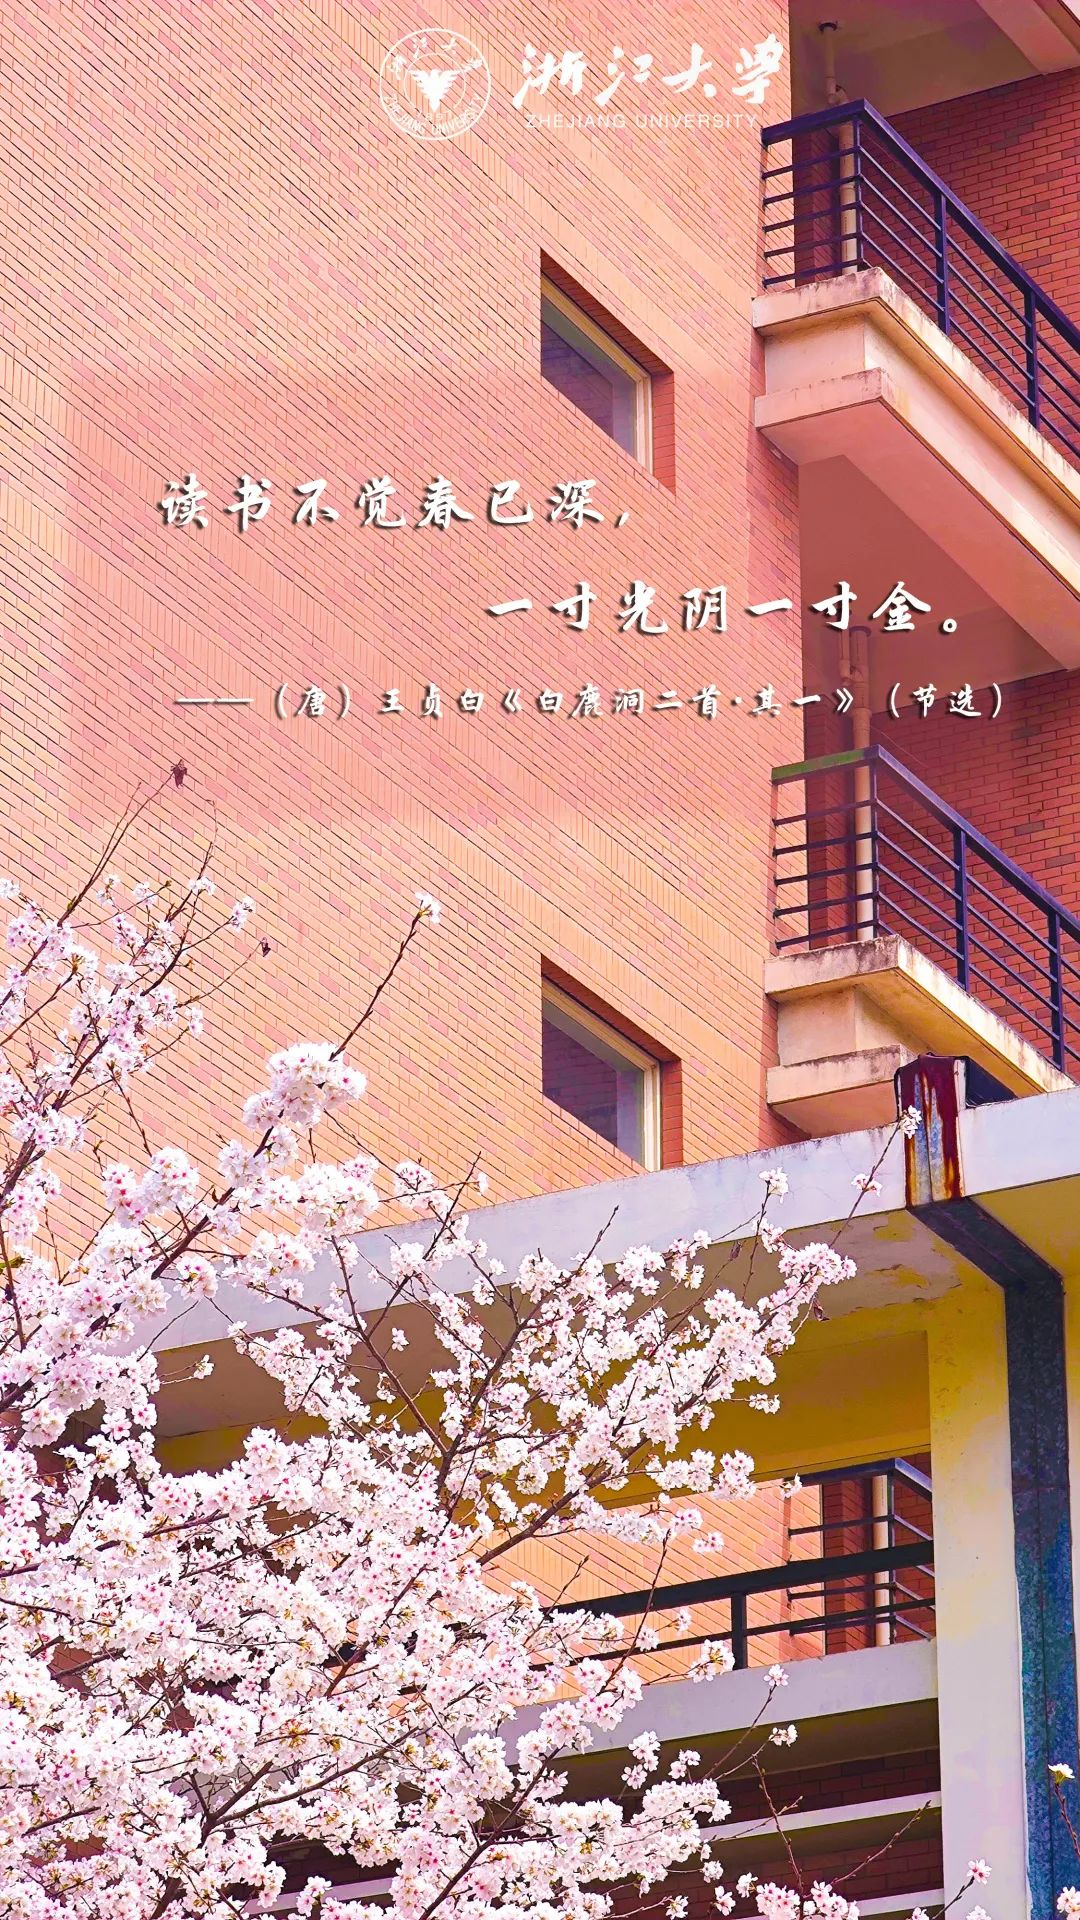
\includegraphics[width=0.3\linewidth]{fig/photo.jpg}
    \caption{
        Every plot must have axes labeled.
    }
    \label{fig:exp_plots}
\end{figure}

\section{Conclusions}
Here you briefly summarize your findings.

% ------------------------------------------------------------------------------
% Reference and Cited Works
% ------------------------------------------------------------------------------
\newpage
\bibliographystyle{IEEEtran}
\bibliography{References.bib}

\end{document}